% !TeX root = ../../tesis.tex

% =============================================================================
\subsection*{Grupo 2: Indicadores de Eficiencia (Tiempo y Forma)}
% =============================================================================

% -----------------------------------------------------------------------
\subsection{Índice de Ruta Directa --- \texorpdfstring{\textit{Detour Factor} ($DI$)}{Detour Factor (DI)}}
\label{subsec:ruta-directa}
% -----------------------------------------------------------------------

\textbf{Fuente principal:} \citet{fortin2016innovative}

\subsubsection{Definición y Fundamentación}

El Índice de Ruta Directa cuantifica qué tan eficiente es la topología de la red
en términos geométricos puros: mide cuánto se alarga un viaje al estar obligado
a seguir la infraestructura real de la red en lugar de desplazarse en línea
recta entre origen y destino. \citet{fortin2016innovative} proponen este
indicador como parte de su método orientado a grafos para caracterizar
sistemáticamente redes de transporte a partir de datos \gtfs{}, donde el
análisis de la topología implica calcular los caminos mínimos entre pares de
nodos y derivar indicadores de desempeño.

Es importante precisar una limitación inherente: el $DI$ no incorpora los pesos
ponderados de las aristas (tiempos reales, frecuencias, factores de congestión),
sino únicamente la ubicación geométrica de los nodos. Es, por tanto, un
indicador de la \termino{eficiencia estructural} de la red ---independiente de
sus condiciones operativas--- y resulta especialmente útil para evaluar el
trazado de nuevas rutas o comparar configuraciones alternativas antes de
incorporar la dinámica de tráfico.

\subsubsection{Fórmula}

\begin{equation}
    DI = \frac{d_{\text{red}}(i,\, j)}{d_{\text{euclidiana}}(i,\, j)}
    \label{eq:detour-factor}
\end{equation}

Donde:
\begin{itemize}
    \item $DI$ = Índice de Ruta Directa (adimensional, siempre $DI \geq 1.0$).
\item $d_{\text{red}}(i, j)$ = Distancia del camino mínimo entre los nodos $i$
    y $j$ medida a lo largo de las aristas del grafo, en km.
    \item $d_{\text{euclidiana}}(i, j)$ = Distancia en línea recta (distancia
    \textit{haversine} para coordenadas geográficas) entre los nodos $i$ y $j$,
    en km.
\end{itemize}

Un valor $DI = 1.0$ representa eficiencia geométrica perfecta (el trayecto en
red coincide con la línea recta). Valores $DI \gg 1.0$ indican que la topología
fuerza a los usuarios a rodeos significativos respecto al desplazamiento ideal.

\begin{figure}[H]
    \centering
    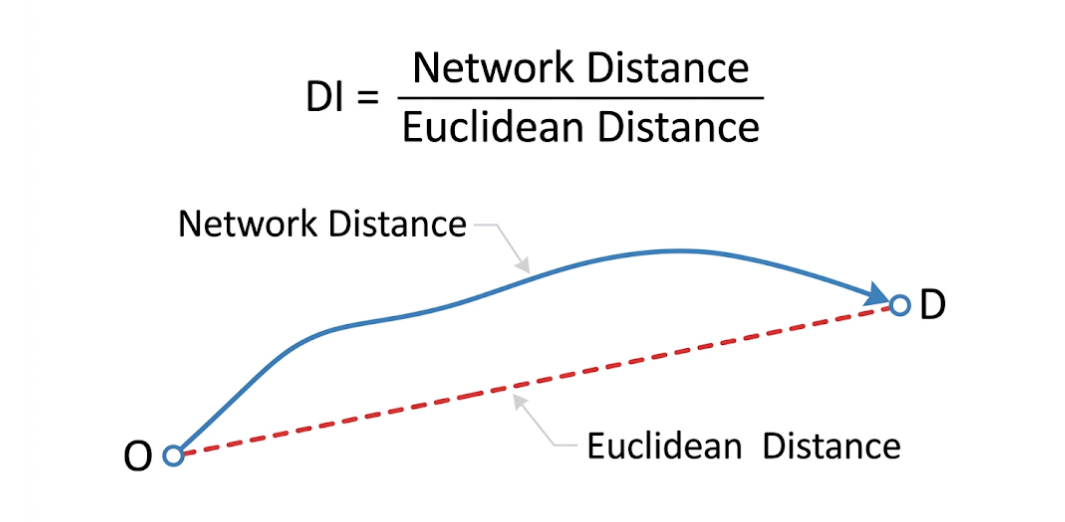
\includegraphics[width=0.65\textwidth]{Figures/Cap3/DistanciaEuclidiana.png}
    \caption[Diagrama del \textit{Detour Factor} $DI$]{Comparación entre la
    distancia en red (arco curvado) y la distancia euclidiana (línea punteada)
    entre origen O y destino D.}
    \label{fig:indicador-DI}
    \fuentefigura{Elaboración propia con base en \citet{fortin2016innovative}.}
\end{figure}

\subsubsection{Ejemplo Práctico: \cdmx{} y Zona Metropolitana}

\begin{table}[H]
    \centering
    \caption{Comparativa del indicador $DI$ antes y después del Anillo Periférico.}
    \label{tab:detour-factor}
    \begin{tabularx}{\textwidth}{X r r r r r}
        \toprule
        \textbf{Par O--D} &
        $d_{\text{eucl.}}$ &
        $d_{\text{red}}$ actual &
        $DI$ actual &
        $d_{\text{red}}$ con Anillo &
        $DI$ con Anillo \\
        \midrule
        Xochimilco $\to$ Santa Fe    & 15\,km & 28\,km & 1.87 & 18\,km & 1.20 \\
        Perisur $\to$ Naucalpan      & 18\,km & 42\,km & 2.33 & 26\,km & 1.44 \\
        Iztapalapa $\to$ Tlalnepantla & 22\,km & 55\,km & 2.50 & 30\,km & 1.36 \\
        \bottomrule
    \end{tabularx}
\end{table}

La implementación computacional de referencia para este indicador se encuentra
en el \autoref{anx:indicadores-implementacion} (§\ref{anx:impl-detour}).

El indicador $DI$ contribuye tanto al Objetivo Específico 2 ---en su papel de
métrica del diagnóstico topológico actual de la red--- como al Objetivo
Específico 5 (§\ref{subsec:obj-especificos}): la reducción del $DI$ entre pares
origen-destino del Tercer y Cuarto Contorno es uno de los efectos directamente
esperables y cuantificables de la incorporación del corredor anillar al grafo de
la \zmvm{}.
